\documentclass[11pt,a4paper,ngerman]{scrreprt}
\usepackage[utf8]{inputenc}

\usepackage{graphicx}

%\usepackage{import}
% imports
\usepackage[automark]{scrpage2}
\usepackage[ngerman]{babel}
%test if available \usepackage{ngerman}
\usepackage[nosectionbib]{apacite}
%\usepackage{splitbib}
%\usepackage{txfonts} 		% Schriftart Times New Roman
%\usepackage{helvet} 		% Schrift Arial
\usepackage{setspace} 		% Zeilenabstand
\onehalfspacing
\usepackage{amsmath}

% embedded code
\usepackage{listings}
\usepackage{color}

\definecolor{dkgreen}{rgb}{0,0.6,0}
\definecolor{gray}{rgb}{0.5,0.5,0.5}
\definecolor{mauve}{rgb}{0.58,0,0.82}

\lstset{frame=tb,
  language=Python,
  aboveskip=3mm,
  belowskip=3mm,
  showstringspaces=false,
  columns=flexible,
  basicstyle={\footnotesize\ttfamily},%{\small\ttfamily},
  numbers=none,
  numberstyle=\tiny\color{gray},
  keywordstyle=\color{blue},
  commentstyle=\color{dkgreen},
  stringstyle=\color{mauve},
  breaklines=true,
  breakatwhitespace=true
  tabsize=3
}

\makeatletter
\setcounter{secnumdepth}{3}
\setcounter{tocdepth}{3}

\makeindex

%Inhaltsverzeichnis bis auf 3 Stufen
\setcounter{tocdepth}{2}

%Kopfzeilen
\pagestyle{scrheadings} %Seitenstil scrheadings verwenden

% Grösse des Textbereiches in der Seite
\setlength{\textwidth}{16cm}
\setlength{\textheight}{22cm}
% Kopf- und Fusszeile, Höhe und Abstand vom Text
\setlength{\headheight}{20pt}
\setlength{\headsep}{0.8cm}
% Linker Seiteneinzug
\setlength{\oddsidemargin}{2.5cm} \addtolength{\oddsidemargin}{-1in}
\setlength{\evensidemargin}{2.5cm} \addtolength{\evensidemargin}{-1in}
% Andere Grössen ausrechnen (vertikal zentrieren)
\setlength{\footskip}{\headsep}
\addtolength{\footskip}{\headheight}
\setlength{\topmargin}{\paperheight}
\addtolength{\topmargin}{-\textheight}
\addtolength{\topmargin}{-\headheight}
\addtolength{\topmargin}{-\headsep}
\addtolength{\topmargin}{-\footskip}
\addtolength{\topmargin}{-2in}
\addtolength{\topmargin}{-0.5\topmargin}

\automark[section]{chapter} %Sektion und Kapitel für Headmark
\setheadsepline{.4pt} %Separate Linie im Kopf
\clearscrheadfoot %Kopf und Fußzeile löschen
\cfoot[\pagemark]{\pagemark} %- mittlere Fusszeile 

\makeatother

\usepackage{babel}
\begin{document}

\date{\today}
\begin{titlepage}
\begin{center}
\vspace*{1.5cm}
\Large \textbf{cp-logic} \\
\Large {Umsetzung der Konzepte aus der Vorlesung \\ \textit{Diskrete Mathematik und Logik} \\ in eine Toolbox für Studierende}
\vspace*{1.5cm}

\vspace*{0.5cm}
\large {Bachelorarbeit}\\
\vspace*{2cm}
\large {Universität Bern \\ Institut für Informatik und angewandte Mathematik \\ Logic and Theory Group (LTG) \\}
\vspace*{2cm}
\large {Eingereicht bei Prof. Dr. Studer}\\
\large {Bern, 22. Mai 2014}\\
\vspace*{1cm}
\large {Adrianus Kleemans [07-111-693]}\\
\large {Seidenweg 14}\\
\large {3012 Bern}\\
\large {077 434 40 44}\\
\large {a.kleemans@gmail.com}\\
\end{center}
\end{titlepage}

\normalsize

\tableofcontents
\clearpage
\renewcommand{\baselinestretch}{1.5}

\chapter{Einleitung}  %=============================================================================================
\section{Abstract}
Anhand dem Skript aus der Vorlesung \textit{Diskrete Mathematik und Logik} wird eine Software realisiert, welche die wichtigsten darin vorgestellten Algorithmen umsetzt und zur Anwendung zur Verfügung stellt. Die Implementierung erfolgte in der Programmiersprache Python und bietet eine grafische Oberfläche, die es erlaubt, Formeln zu definieren und mit einer Palette an Funktionen zu manipulieren und als Text oder auch grafisch auszugeben.

\section{Motivation}
Im Skript \textit{Discrete Mathematics and Logic} von Prof. G. Jäger zur gleichnamigen Vorlesung wird ein Katalog an Verfahren und Begriffen eingeführt, um Formeln zu definieren, zu vereinfachen, in bestimmte Normalformen zu bringen (z.B. konjunktive Normalform oder Negationsnormalform) oder auf Erfüllbarkeit zu testen (z.B. PSC-SAT, Resolution, Deduktionsketten). Um den Zugang zu diesen Konzepten zu erleichtern, war meine Motivation, eine einfache Umgebung zur Verfügung zu stellen, um den Studierenden des Kurses einen schnellen Einstieg zu ermöglichen und erlernte Verfahren gleich testen zu können. Das Modul \textbf{cp-logic} soll diese Ansprüche erfüllen und auf einfache Art und Weise den Zugang ermöglichen.

\section{Ziele und Fokus}
Abgeleitet aus der Motivation entstand eine Zielsetzung, welche sich hauptsächlich aus zwei Teilen zusammensetzt:
\begin{enumerate}
 \item Die vorgestellten Funktionen aus dem vorgestellten Skript implementieren und
 \item in einer einfachen Art und Weise den Benutzern zur Verfügung stellen.
\end{enumerate}
Diese lassen sich noch weiter spezifizieren. Zum Beispiel sollte es möglich sein, vorgestellte Funktionen Eins zu Eins aus dem Skript eingeben zu können und dabei das richtige Resultat zu erhalten. So sollte es z.B. möglich sein, 
\begin{equation}
\text{sufo} (p_0 \wedge (\neg p_1 \vee p_2))
\end{equation}
einzugeben (\textit{sufo} ist der Befehl für die \textit{subformulas}, also die ``Untermengen'' der Formel) und die Menge 
\begin{equation}
\{ p_0, p_1, p_2, \neg p_1, (\neg p_1 \vee p_2), p_0 \wedge (\neg p_1 \vee p_2) \}
\end{equation}
zu erhalten. Weiter sollte eine benutzerfreundliche Eingabe über ein GUI ermöglicht werden, und damit einer Reihe von kleineren Anforderungen Rechnung getragen werden:
\begin{itemize}
 \item Anzeige eines Verlaufs, d.h. von bereits durchgeführten Eingaben
 \item verschachtelbare Funktionen
 \item Metavariablen zur Speicherung von Formeln, damit Formeln nicht mehrmals eingegeben werden müssen
 \item Unterstützung durch das GUI bezüglich Funktionalität und Eingabe (z.B. mit Menü-Einträgen)
\end{itemize}
Da die Software am Ende dazu dienen soll, Studierende zum Ausprobieren zu animieren, liegt der Fokus mehr auf der Demonstration, Fehlererkennung und einer einfachen Darstellung von Algorithmen als auf einem Performance-optimierten Ansatz (die Folgen daraus werden kurz in Abschnitt \ref{section:einschraenkungen} angesprochen). Das heisst, statt korrekte Eingaben zu erwarten und diese optimiert zu verarbeiten bietet die Applikation eine weitreichende Fehlererkennung (z.B. was die Definition einer ``korrekten'' Formel angeht) mit detailliertem Feedback für den User. 

Die Eingabe soll dabei so frei wie möglich gestaltet werden, und es werden sowohl reine ASCII- sowie Unicode-Eingaben unterstützt, sogar gemischte Eingaben sollten kein Problem darstellen. Die Ausgabe sollte einheitlich immer in Unicode erfolgen.

\section{Wahl der Technologie}
Aus den abzubildenden Verfahren ergibt sich direkt der Anforderungskatalog, welcher berücksichtigt werden musste:
\begin{itemize}
 \item Vollständige Unicode-Unterstützung (zur Abbildung von Zeichen wie $\wedge$, $\vee$, $\neg$ etc.)
 \item Datenstrukturen für Formeln, verschachtelte Listen, binäre Bäume (für Deduktionsketten), assoziative Arrays (dicts)
 \item Lesbarkeit des Codes, niedrige Komplexität (Erweiterbarkeit ermöglichen)
 \item Grafische Darstellung einer Konsolen-ähnlichen Anwendung
 \item Grafische Darstellung von Deduktionsketten
\end{itemize}
Als Programmiersprache, welche alle Anforderungen erfüllt, wurde schliesslich \textbf{Python} ausgewählt, welche vor allem was Unicode und die Lesbarkeit des Codes angeht grosse Vorteile aufweist.

\section{Entwicklungsentscheide} % <-> Ziele
Um die festgelegten Ziele zu erfüllen, wurde nach folgenden Programmierparadigmen gearbeitet:
\begin{itemize}
\item \textbf{Test driven design (TDD)} \\
Da schon im Vorfeld ein Grossteil der Funktionalität, die am Ende angeboten werden sollte, bekannt war, wurde zu einem grossen Teil mit Tests gearbeitet. Diese schlugen zuerst fehl, die Entwicklung wurde jedoch durch diese vorangetrieben und dienten als Prüfstein dazu, wie weit die Erfüllung der Ziele schon fortgeschritten war.

\item \textbf{Responsibility driven design} \\
Nebst den Tests war jedoch auch klar, dass die Entwicklung objektorientiert sein sollte. Aus den verschiedenen Objekten ergaben sich verschiedene Verantwortlickeiten, wie z.B. für die \textit{Formula}-Klasse, welche eine Formel darstellt, oder die \textit{Tools}-Klasse, welche einige Funktionen zur Verfügung stellt.
Mehr zu den spezifischen Verantwortungen der Klassen lässt sich in Abschnitt \ref{section:verantwortlichkeiten} finden.

\item \textbf{Use cases} \\
Durch das Festlegen diverser Use Cases wurde evaluiert, wie die Eingabe, Manipulation und Anzeige des Resultats erfolgen sollte. Die verschiedenen Anforderungen der Eingabe wurden dabei festgehalten und in einen durchgängigen Ablauf integriert, wie genau die Verarbeitung einer Eingabe erfolgen sollte. Dies wird in Abschnitt \ref{section:inputverarbeitung} dargestellt.
\end{itemize}

\section{Einschränkungen}
\label{section:einschraenkungen}
Nebst den bereits erwähnten Einschränkungen, was die Performance angeht, wurde auch auf gewisse Teile des Skripts verzichtet. Dies umfasst die doppelte Implikation $\leftrightarrow$, welche zwar als abgekürzte Schreibweise eingeführt wird, aber danach im Skript nicht mehr vorkommt. Auf Theorien wurde auch verzichtet, da eine äquivalente Repräsentation (auch im Sinne von Kapitel 2.9, ``Adding Theories to PSC'') den Rahmen dieser Arbeit sprengen würde. Das Hilbert-Kalkül wurde bewusst weggelassen, da im Sinne der Vorlesung der Fokus auf PSC (Deduktionsketten) und Resolution lag.

\chapter{Das Paket cp-logic} %=============================================================
\section{Funktionalität}
\subsection{Generelle Funktionsweise}
Über eine konsolenartige Eingabe können in ein Textfeld Formeln und anzuwendende Funktionen direkt eingegeben werden.

\begin{figure}[ht]
\centering
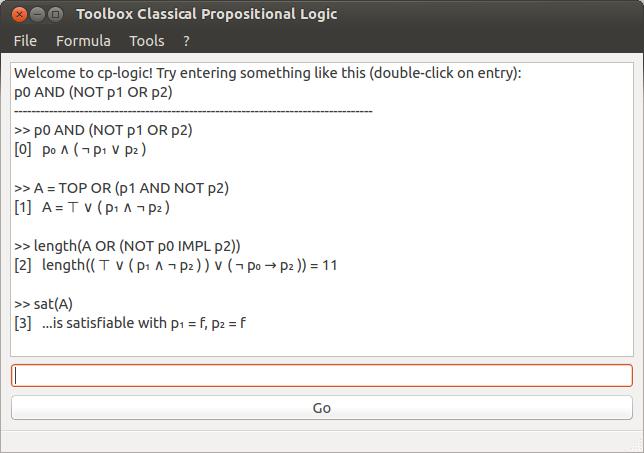
\includegraphics[width=.9\linewidth]{pics/gui.png}
\end{figure}

Dabei wird im oberen Bereich ein Verlauf der letzten Eingaben angezeigt, welche die aktuelle \textbf{Session} ausmachen. So können z.B. Befehle per Doppelklick in das Eingabefeld kopiert werden oder auch auf bereits definierte Metavariablen zurückgegriffen werden (im obigen Beispiel die Variable \textit{A}). % , siehe dazu auch Abschnitt \ref{section:metavariables}

\subsection{Formelobjekte}
Wird eine Formel eingegeben, so wird die Eingabe analysiert und ein neues Objekt der Klasse \textit{formula} erstellt. Hier werden diverse Annahmen geprüft, dass eine gültige Formel eingegeben wurde.

Ein Beispiel dafür ist die Bedingung, dass atomare Propositionen immer einen Index benötigen und zudem über Konjunktionen verknüpft sein müssen (Ausschnitt aus \textit{Formula.check()}):
\begin{lstlisting}
# checking for propositions
parts = f.split()
for i in range(len(parts)):
    if parts[i] == 'p':
        raise FormulaInvalidError('propositions need an index')
    if i < len(parts)-1 and parts[i].startswith('p') and parts[i+1].startswith('p'):
        raise FormulaInvalidError('propositions need to be connected with a conjunction')
\end{lstlisting}
Eine ausführliche Liste mit Beschreibungen aller Fehlerarten findet sich im Abschnitt \ref{section:fehlerbehandlung}. Danach werden nacheinander alle anderen Formen berechnet, von \textit{pedantic} über \textit{NNF} bis hin zur \textit{CNF}. Diese werden im nächsten Abschnitt noch kurz erläutert.

Nach der Erstellung eines (oder je nach Eingabe mehrerer) Formelobjekts werden die entsprechenden Funktionen ausgeführt und das Resultat wird dem Benutzer als unterster Eintrag in seinem Verlauf angezeigt.

\subsection{Übersicht Normalformen und Funktionen}
\begin{figure}[ht]
\centering
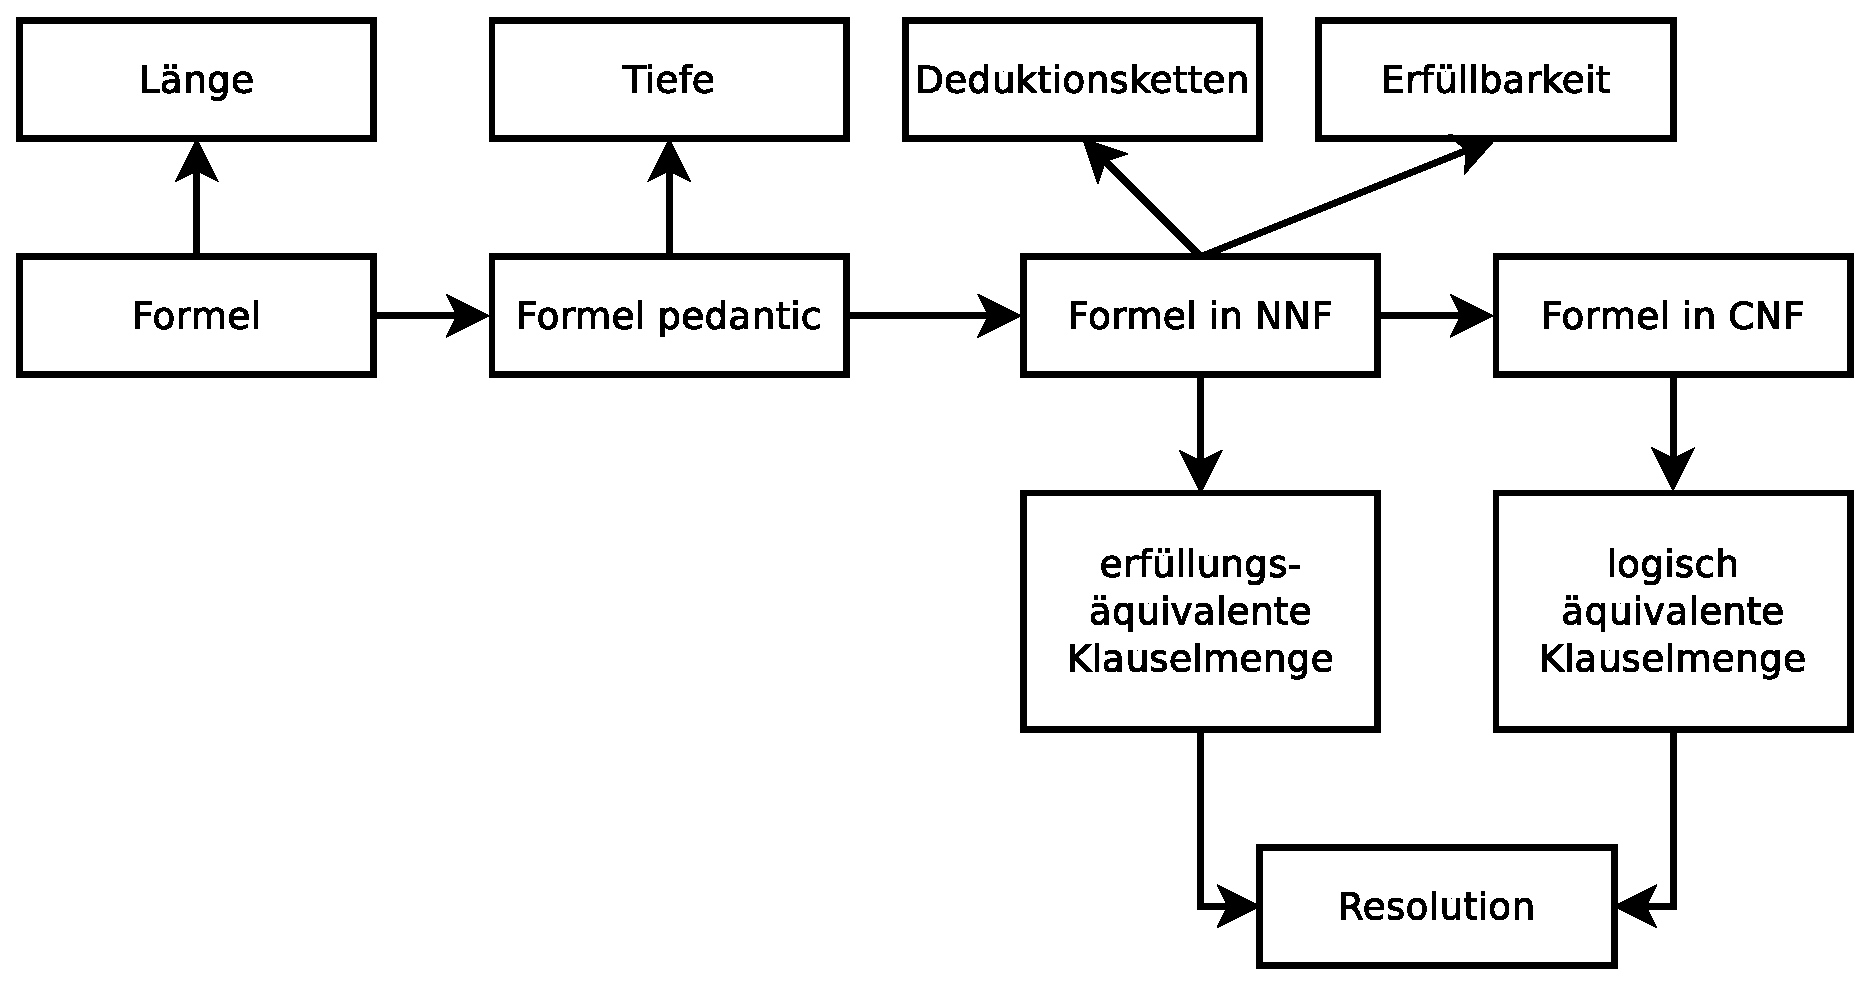
\includegraphics[width=.9\linewidth]{pics/Normalformen.eps}
\end{figure}

Da verschiedene Funktionen je nach dem eine andere Form einer Formel benötigen, damit die Berechnung funktioniert, muss für jede Formel ihre Normalformen berechnet werden. Diese Übersicht über die Normalformen zeigt die zentralen Funktionen, die im Fokus der Arbeit stehen, allen voran die Deduktionsketten und die Resolution.

Viele Funktionen können auf eine Formel angewendet werden, egal in welcher Form sie sich befindet, z.B. ist sowohl \texttt{length(p0 IMPL p1)} als auch \texttt{length(nnf(p0 IMPL p1))} (entspricht \texttt{length(NOT p0 OR p1)}) möglich, was jedoch auch zu anderen Resultaten führt (3 bzw. 4 in diesem Fall).

\subsection{Funktionsumfang}
Im Folgenden werden die wichtigsten Funktionen mit je einem Beispiel dazu vorgestellt.
\begin{itemize}
\item \textbf{length()} - gibt die Länge einer Formel an \\
\texttt{>> length(p0 OR NOT p1)} \\
\texttt{[0] length($p_0 \vee \neg p_1$) = 4}

\item \textbf{sufo()} - berechnet die Subformulas einer Formel \\
\texttt{>> sufo(p0 OR (NOT p1 AND p2))} \\
\texttt{[0] Found the following 6 subformulas: \\
$p_0$ \\
$p_1$ \\
$p_2$ \\
$\neg p_1$ \\
$( \neg p_1 \wedge p_2 )$ \\
$p_0 \vee ( \neg p_1 \wedge p_2 )$}

\item \textbf{latex()} - zeigt die Formel in \LaTeX-Notation an \\
\texttt{>> latex(p0 OR NOT p1)} \\
\texttt{[0] p\_0 \textbackslash vee \textbackslash neg p\_1}

\item \textbf{pedantic()} - zeigt die pedantische Form der Formel an \\
\texttt{>> pedantic(p0 AND p1 AND p2 AND NOT p3)} \\
\texttt{[0] $( ( p_0 \wedge p_1 ) \wedge p_2 ) \wedge \neg p_3$}

\item \textbf{nnf()} - zeigt die Negationsnormalform der Formel an \\
\texttt{>> nnf(p0 IMPL NOT (NOT p1 OR p2))} \\
\texttt{[0] $\neg p_0 \vee ( p_1 \wedge \neg p_2 )$}

\item \textbf{cnf()} - zeigt die konjunktive Normalform der Formel an \\
\texttt{>> cnf(p0 IMPL NOT (NOT p1 OR p2))} \\
\texttt{[0] $( \neg p_0 \vee p_1 ) \wedge ( \neg p_0 \vee \neg p_2 )$}

\item \textbf{sat()} - prüft, ob eine Formel erfüllbar ist \\
\texttt{>> sat(p0 IMPL NOT (NOT p1 OR p2))} \\
\texttt{[0] ...is satisfiable with $p_0$ = f, $p_1$ = f, $p_2$ = f}

\item \textbf{clause\_set()} - zeigt die entsprechende Klauselmenge zu einer Formel an \\
\texttt{>> clause\_set((p0 AND NOT p1) OR (p1 AND NOT p2))} \\
\texttt{[0] Found the following 4 clauses: \\
$\{p_0, p_1\}$ \\
$\{\neg p_1, p_1\}$ \\
$\{p_0, \neg p_2\}$ \\
$\{\neg p_1, \neg p_2\}$}

\item \textbf{evaluate()} - gibt an, ob eine Formel ohne Propositionen zu \textit{wahr} oder \textit{falsch} evaluiert \\
\texttt{>> evaluate(TOP OR (TOP AND BOTTOM AND TOP))} \\
\texttt{[0] $\top \vee ( \top \wedge \bot \wedge \top )$ evaluates to True}

\item \textbf{resolution()} - führt das Resolutions-Verfahren an einer Formel durch \\
\texttt{>> resolution((p0 AND NOT p1) OR (p1 AND NOT p2))} \\
\texttt{[0] Found the following 4 clause sets: \\
$p_0, p_1$ \\
$\neg p_1, p_1$ \\
$p_0, \neg p_2$ \\
$\neg p_1, \neg p_2$ \\\\
Empty set not found ==> satisfiable.}

\item \textbf{dchains()} - berechnet die Deduktionsketten mehrerer Formeln und prüft diese auf Gültigkeit \\
\texttt{>> dchains(BOTTOM OR TOP, p2 AND (NOT p2 OR p3), p1 AND (p2 OR p4))} \\
\texttt{[0] Chain is valid in PSC.}\\
Dabei werden die Deduktionsketten als Baumstruktur grafisch dargestellt.
\begin{figure}[ht]
\centering
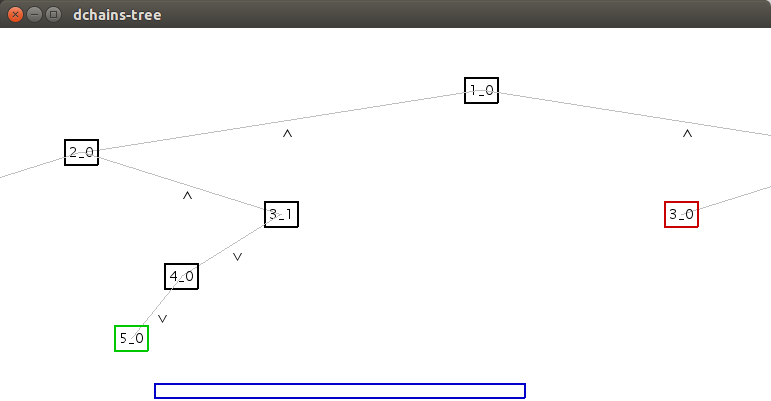
\includegraphics[width=.9\linewidth]{pics/tree2a}
\end{figure}
\end{itemize}
\newpage \noindent Mit Klick auf einen Knoten kann die entsprechende Kette angezeigt werden. Die Farben der Knoten haben folgende Bedeutung:
\begin{itemize}
\item \textbf{Schwarz} heisst, dass die entsprechende Sequenz noch reduzierbar ist
\item \textbf{Rot} heisst, dass die entsprechende Sequenz irreduzibel und kein Axiom ist
\item \textbf{Grün} heisst, dass die Sequenz ein Axiom (\textit{True} oder \textit{Identity}) von PSC ist
\end{itemize}

\section{GUI}
\subsection{Übersicht}
Die Oberfläche ist recht einfach aufgebaut und besteht aus folgenden Bestandteilen:

\begin{figure}[ht]
\centering
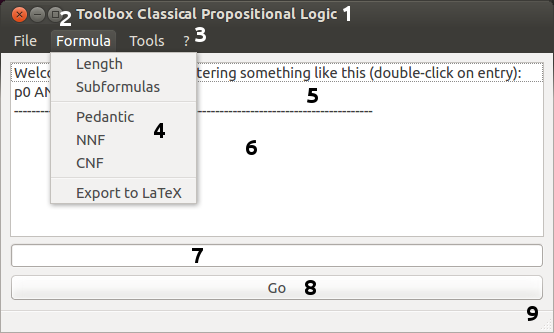
\includegraphics[width=.7\linewidth]{pics/gui2.png}
\end{figure}

\begin{enumerate} 
\item Titelleiste mit Anzeige
\item Steuerelemente zum schliessen, minimieren, maximieren des Fensters
\item Hauptmenüstruktur
\item Untermenüs zum Anwählen von Funktionen
\item kurze Einleitung mit Beispiel
\item Verlauf der Eingaben
\item Texteingabefeld zur Eingabe der Formeln und Funktionen
\item Button zum Absenden der Eingabe, löst die Verarbeitung aus
\item Steuerelement zur Skalierung des Fensters
\end{enumerate}

\subsection{Technologie}
Um die Anwendung plattformunabhängig zu gestalten, wurde aus mehreren Varianten schliesslich \textbf{Pyside} gewählt, die Python-Version von \textbf{QT}. Das GUI wurde im \textit{QT Designer} erstellt und mit Hilfe eines Skripts in Python-Code übersetzt.
\begin{figure}[ht]
\centering
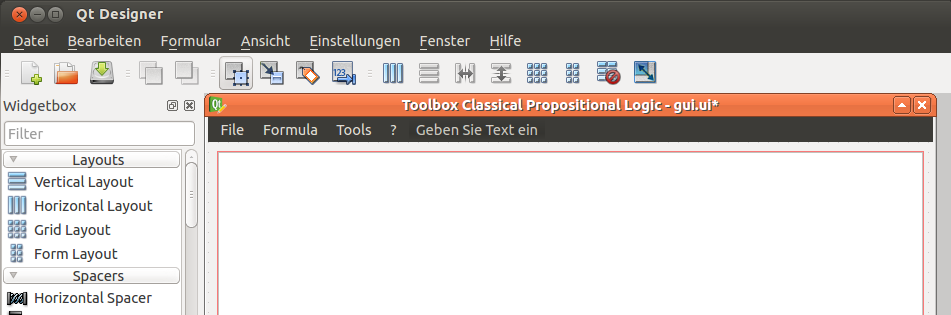
\includegraphics[width=.9\linewidth]{pics/designer.png}
\end{figure}
Das Interface ist dabei als UI-File gespeichert, eine spezifisch auf Oberflächen angepasste XML-Datei. Dort wird das Fenster und all seine Komponenten wie Menü-Struktur, Steuerelemente wie Labels und das Textfeld definiert. Auch die Verknüpfungen zu den entsprechenden Python-Funktionen werden hier festgelegt, z.B. was geschehen soll, wenn auf einen Eintrag in der Liste geklickt oder wenn Enter gedrückt wird.

\subsection{Design decisions}
Beim Aufbau des Interfaces wurde versucht, die folgenden Kriterien zu berücksichtigen:
\begin{itemize}
 \item \textbf{Nachvollziehbarkeit} \\
 Ein wichtiger Faktor bei der Anwendung der Formeln ist die Nachvollziehbarkeit, also zu wissen, was bereits eingegeben wurde, und wieder rasch darauf zugreifen zu können. Eine solche Session soll einen Zwischenspeicher enthalten, der über Metavariablen realisiert wurde. Damit ist es schnell möglich, aufbauend auf einfachen Ausdrücken, komplexere Formeln zu realisieren. 
 
 \item \textbf{Substitutivität} \\
 Nebst der kurzen Einführung in den ersten Zeilen, wo bereits ein Beispiel dargestellt wird, sind Funktionen über die direkte Eingabe und die Menüstruktur zugänglich. \\
 Auch die Eingabe selbst kann über Standard-ASCII-Zeichen oder aber auch direkt als Unicode (\textit{UTF-8}) erfolgen. Die beiden Formatierungen können gemischt werden und sollten so eine möglichst unkomplizierte Eingabe ermöglichen.
 
 \item \textbf{Grafische Darstellung} \\
 Die Anwendung sollte einerseits als eigenständig wahrgenommen werden und trotz dem konsolen-ähnlichen Aufbau eine eigene Menüstruktur besitzen, und andererseits grafische Darstellungen ermöglichen, wie dies bei den Deduktionsketten realisiert wurde.
 
 \item \textbf{Ästhetik} \\
 Das GUI wurde bewusst schlicht gehalten und basiert in jedem Fall auf den systeminternen Darstellungskomponenten, da QT als plattformübergreifende Bibliothek darauf zurückgreift.  Das heisst, unabhängig von der Wahl des Betriebssystems sollten immer aktuelle Darstellungsformen verwendet werden.
 %evtl. Screenshots Windows, Linux, MAC
 
 \item \textbf{Skalierbarkeit} \\
 Das Design wurde so gewählt, dass alle Fenster (auch die grafische Darstellung der Deduktionsketten) vollständig skalierbar sind und es so dem Benutzer erlauben, je nach Bedarf und Bildschirmgrösse eine passende Einstellung zu finden. Auch was die Eingabe angeht ist das Haupteingabefenster skalierbar, so sind beide Richtungen über Scrollen bedienbar, was sowohl sehr viele (vertikaler Scrollbalken) als auch sehr lange Formeln (horizontaler Scrollbalken) zulässt.
\end{itemize}

\section{Klassenbeschreibung, UML}
\label{section:verantwortlichkeiten}

\begin{figure}[h]
\centering
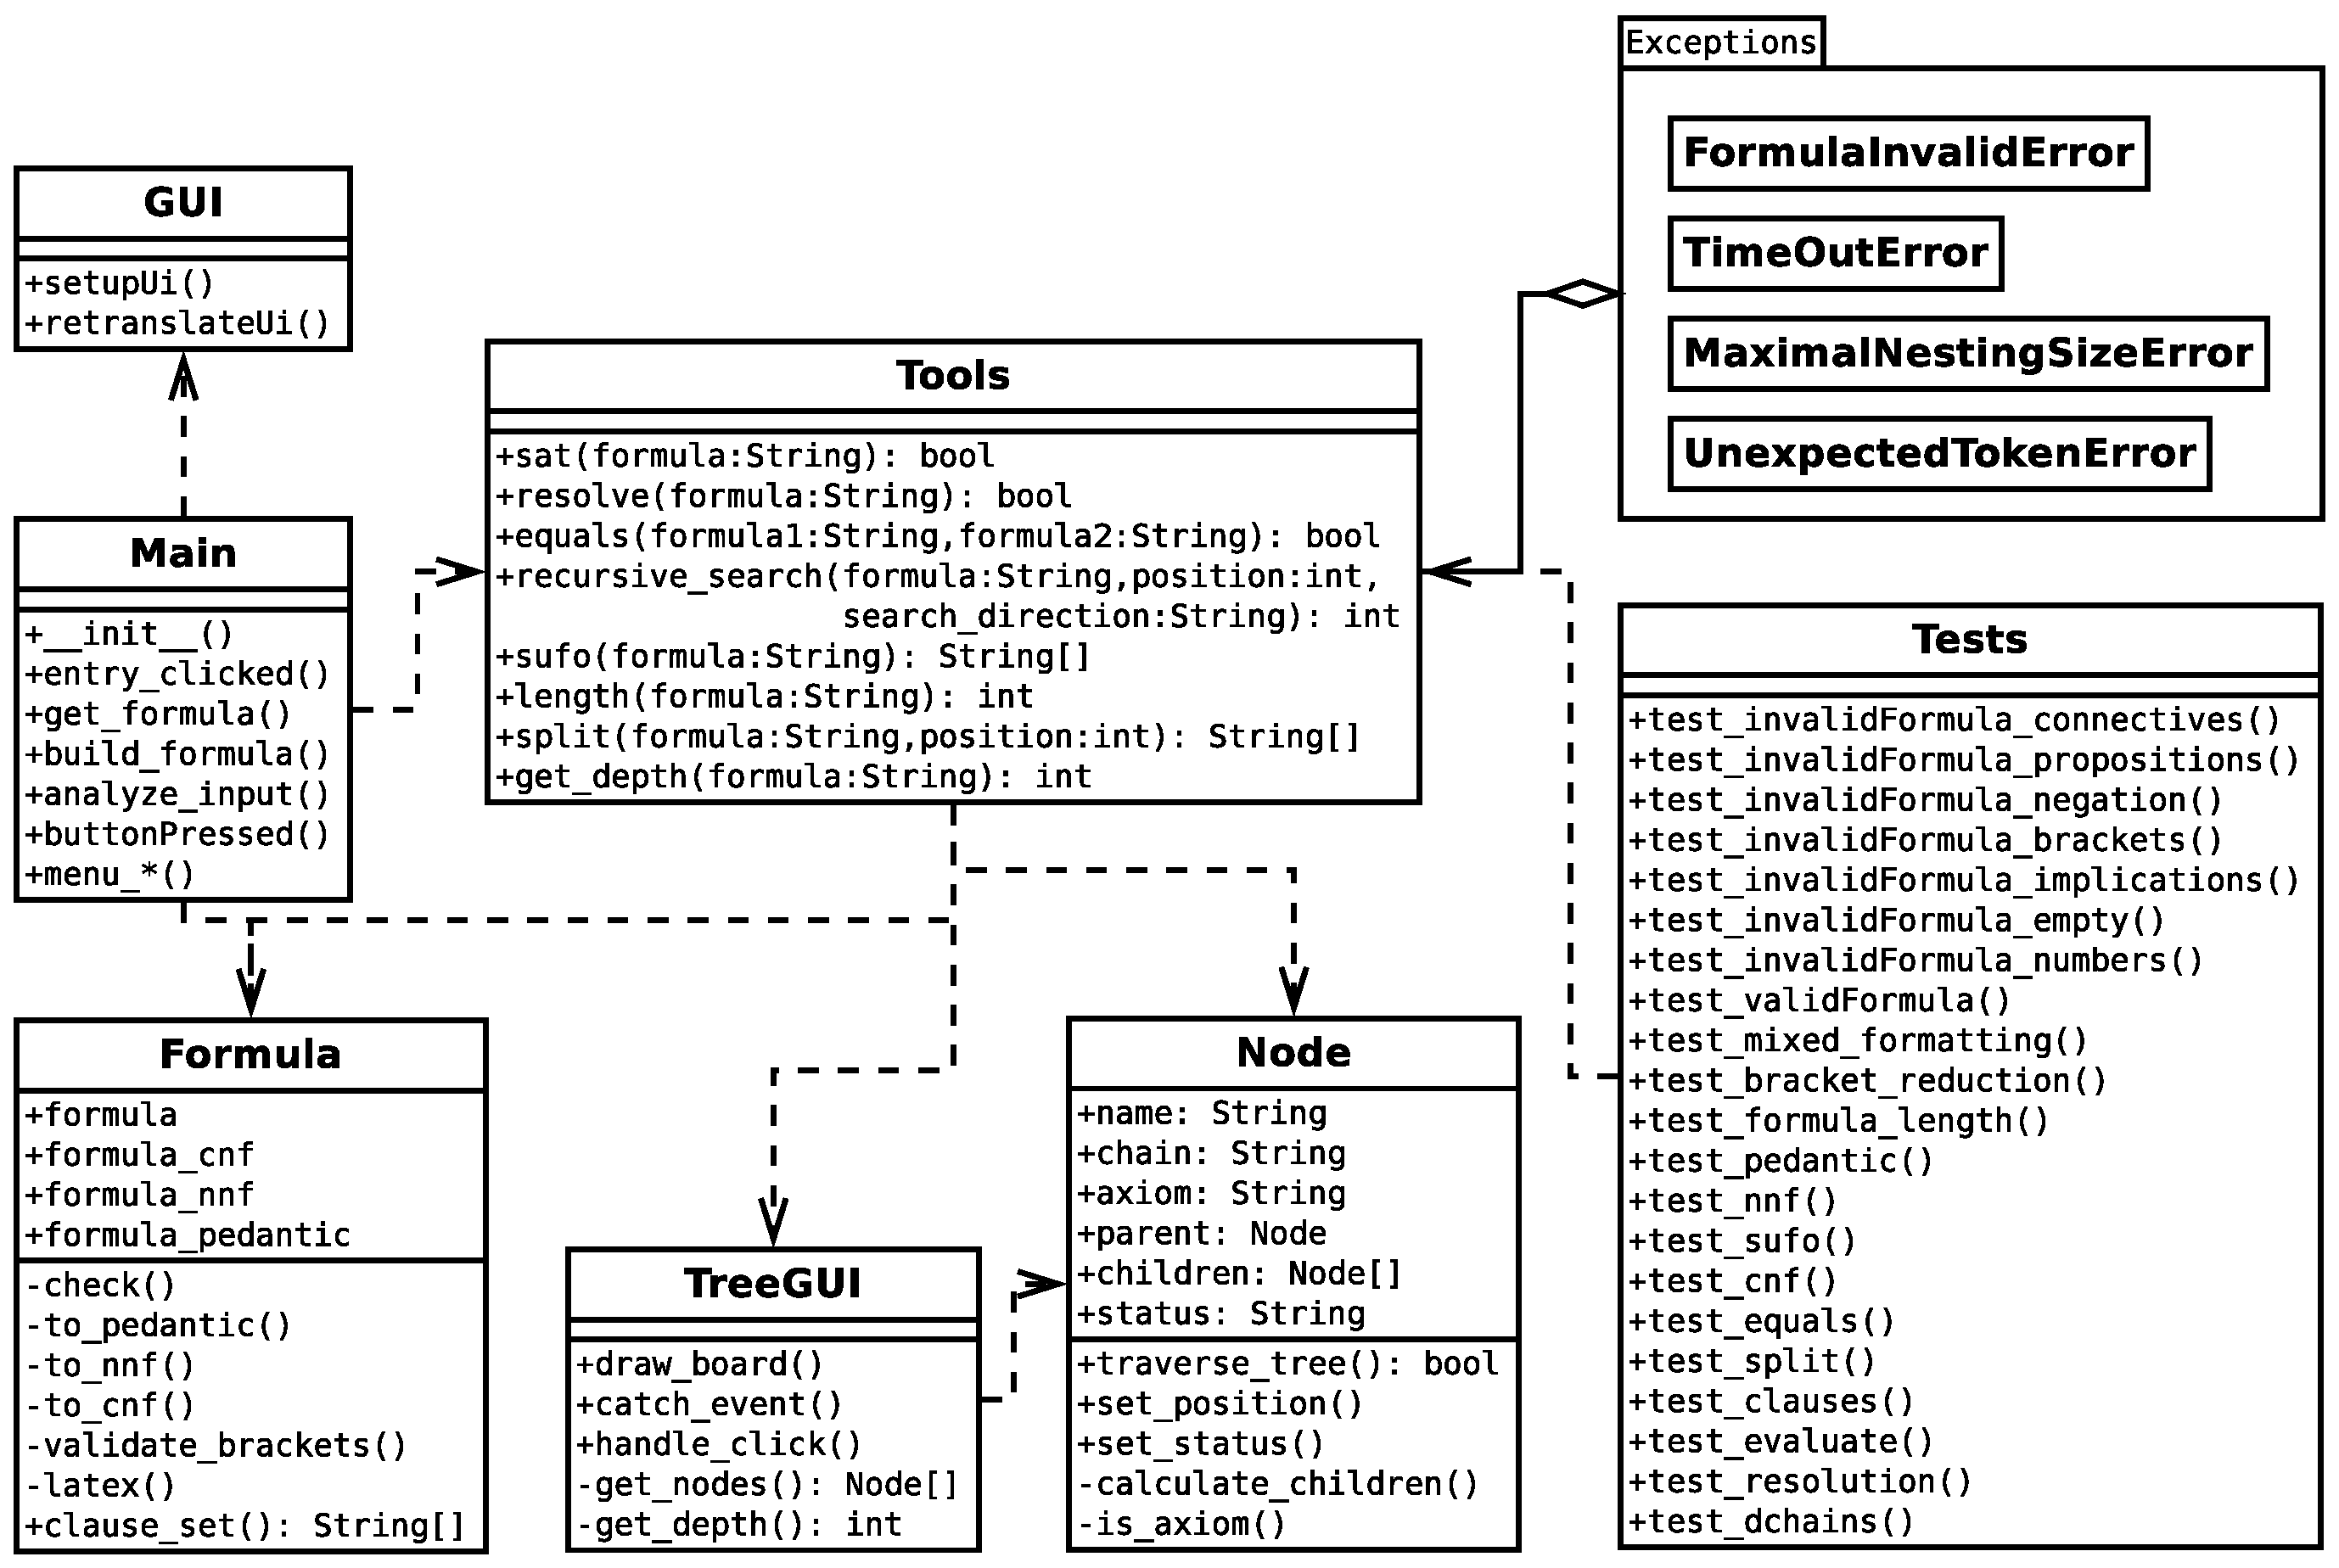
\includegraphics[width=.95\linewidth]{pics/UML.eps}
\end{figure}

\begin{itemize}
 \item \textbf{Main} \\
 Steuerungsklasse, welche das GUI lädt, die anderen Klassen vorbereitet und die Eingabe verarbeitet.
 
 \item \textbf{GUI} -
 Stellt die grafische Oberfläche dar. Präsentiert sich dem Benutzer und gibt die Eingaben weiter an die Main-Klasse.
 
 \item \textbf{Formula} -
 Repräsentiert eine einzelne Formel und beinhaltet einige Formel-nahe Funktionen, wie die Umwandlung in andere Normalformen oder Formate.
 
 \item \textbf{Tools} -
 Enthält die Algorithmen, die auf die Formula-Klasse angewendet werden können. Beispiele dazu sind Erfüllbarkeitstest, Deduktionsketten und Resolution.

 \item \textbf{TreeGUI} -
 Stellt das GUI für die Deduktionsketten dar. Ist zuständig für die Positionierung der Knoten und deren Darstellung auf der Bildfläche. Verarbeitet Eingaben wie Mausklicks und löst die entsprechenden Aktionen aus (z.B. Anzeige der zugehörigen Formel).
 
 \item \textbf{Node} -
 Stellt einen Knoten im Deduktionsketten-Baum dar. Verwaltet die eigene Formel mit den zugehörigen Eigenschaften und enthält Verknüpfungen auf ihre Kinderknoten.
 
 \item \textbf{Tests} -
 Enthält sämtliche Unit Tests, inkl. Regressionstests, für alle Klassen, die getestet werden müssen.
\end{itemize}

\section{Algorithmen}
\subsection{Input-Verarbeitung}
\label{section:inputverarbeitung}
Die Verarbeitung einer Eingabe wird grundsätzlich in zwei Möglichkeiten unterteilt: \textbf{Zuweisung} und \textbf{Funktion}. Dabei wird anhand einer Überprüfung ob das ``$=$''-Zeichen in der Formel vorkommt unterschieden, wie die Eingabe weiter verarbeitet werden soll.
\begin{figure}[ht]
\centering
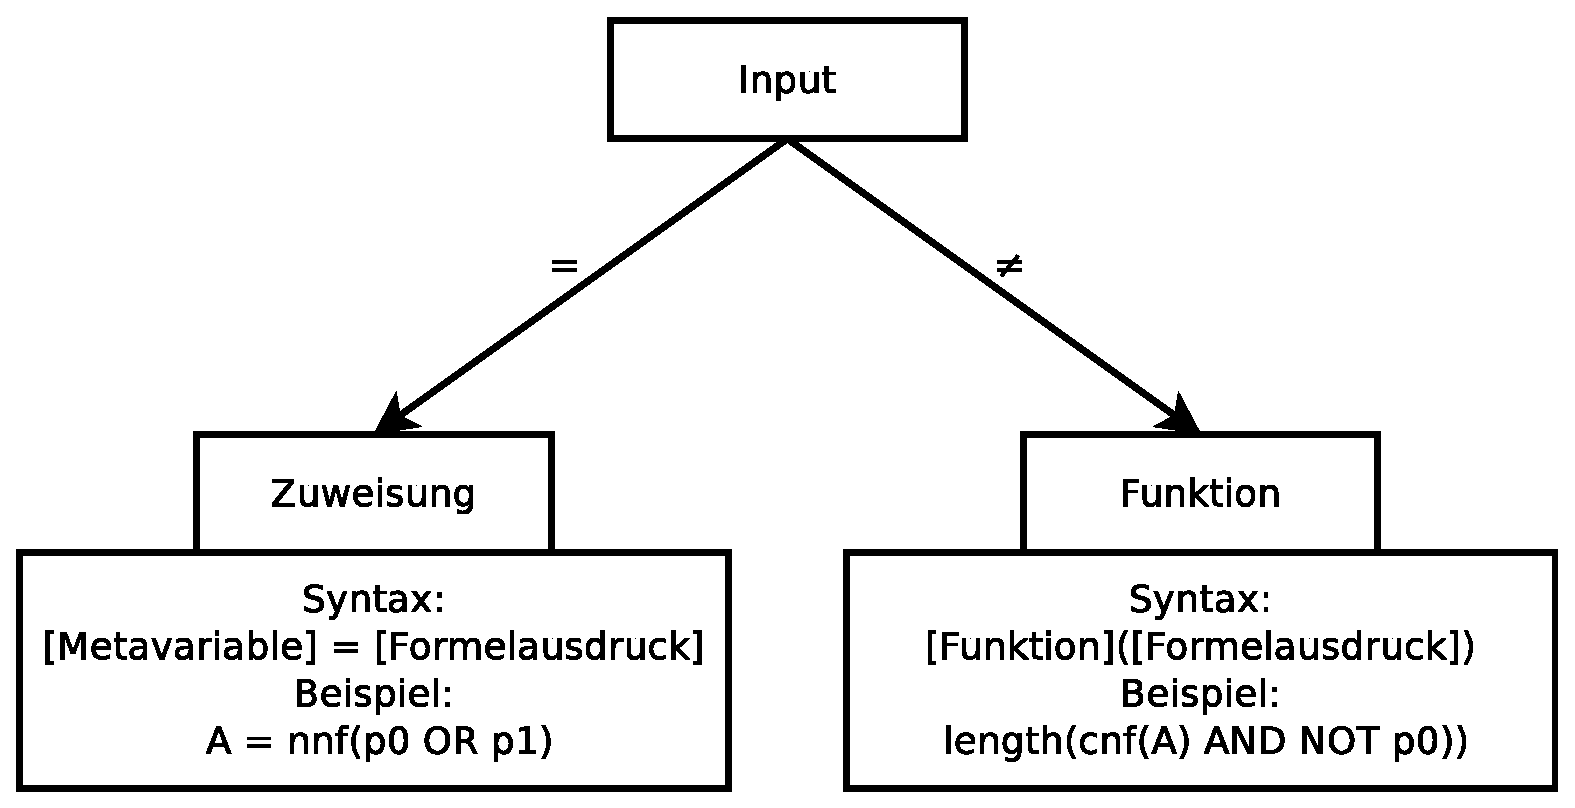
\includegraphics[width=.9\linewidth]{pics/input.eps}
\end{figure}
Dabei kann der beschriebene \textbf{Formelausdruck}, der bei beiden Eingabearten eine wichtige Rolle spielt, aus verschiedensten Elementen bestehen, also einfachen Formelteilen (z.B. \texttt{p0 OR NOT p1}), Metavariablen (z.B. \texttt{A}) oder bereits angewandte Form-Manipulatoren (z.B. \texttt{nnf(A)} oder \texttt{cnf(NOT p0 IMPL p1)}). Dieser Formelausdruck wird schlussendlich zu einer einzigen Formel umgewandelt und so weiter verarbeitet. Ein Beispiel für ein etwas komplexeren Formelausdruck, bestehend aus 4 Einzelteilen, stellt der folgende Ausdruck dar. Hier werden zuerst die Normalformen der einzelnen Komponenten berechnet und am Schluss das Ganze zusammengesetzt, wie dies im Resultat sichtbar ist: \\\\
\texttt{>> length(nnf(A) AND pedantic(p2 IMPL p1) AND NOT p1 AND cnf(NOT p0 AND B))}\\
\texttt{[0] length($p_0 \wedge p_1 \wedge p_2 \rightarrow p_1 \wedge \neg p_1 \wedge \neg p_0 \wedge ( p_0 \wedge p_1 )$) = 17}

\subsection{Exakte Form (\textit{pedantic})}
\label{section:pedantic}
Die ``pedantische'' (englisch: \textit{pedantic}) Version einer Formel ist noch keine Normalform, doch weist sie schon stärkere Einschränkungen auf als eine beliebige Formel. Um die Formel manipulieren zu können, wird ein Verfahren angewendet, welches für jede Stelle der Formel die sogenannte Tiefe (\textit{depth}) ermittelt. Bei jeder Verschachtelung steigt diese an, beginnend mit Ebene 0.
\begin{figure}[ht]
\centering
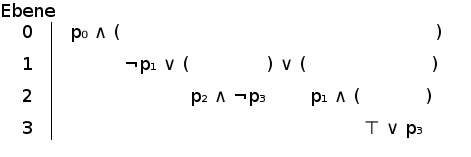
\includegraphics[width=.7\linewidth]{pics/levels}
\end{figure}
Öffnet sich eine neue Klammer, so erhöht sich die Ebenentiefe (\textit{level}) um 1, bei einer schliessenden Klammer verringert sie sich. Dieses Konzept wird hier und auch später noch dafür benötigt, damit bestimmte Algorithmen effizient laufen und nur den Teil der Formel berücksichtigen, der momentan im Fokus steht.
%\newpage
Zu den aufgelisteten Regeln gelten hier, die im Abschnitt 2.1 des Vorlesungsskriptes vorgestellt werden, zusätzlich zwei Regeln, die eingeführt werden mussten, da im Skript noch Spielraum offen gelassen wird.

\begin{enumerate}
 \item \textbf{$\neg$ hat Vorrang vor $\wedge$, $\vee$ und $\rightarrow$} \\
 Diese Regel wird implizit umgesetzt, indem Negationen immer zur Proposition (oder $\top$, $\bot$) gezählt werden, statt als Konjunktion zu gelten.
 
 \item \textbf{$\wedge$ und $\vee$ haben Vorrang vor $\rightarrow$} \\
 Hier werden die Klammern so gesetzt, dass klar ist, das mit $p_0 \wedge p_1 \rightarrow p_2$ der Ausdruck $(p_0 \wedge p_1) \rightarrow p_2$ gemeint ist.
 
 \item \textbf{$\wedge$ und $\vee$ auf gleicher Ebene werden von links nach rechts interpretiert} \\ 
 Ausgehend von der binären Natur einer Konjunktion können $\wedge$ und $\vee$ immer nur genau 2 Ausdrücke miteinander verknüpfen. Eine Verknüpfung in der Art $p_0 \vee p_1 \vee p_2$ ist deshalb streng genommen ungültig, da nicht klar ist, ob dies entweder $(p_0 \vee p_1) \vee p_2$ oder $p_0 \vee (p_1 \vee p_2)$ entspricht.
 
 Deshalb werden Klammern eingefügt, und aus den zwei Möglichkeiten (rechts nach links oder umgekehrt) wurde die Variante genommen, die der Leserichtung entspricht, also von links nach rechts.
 
 \item \textbf{Unnötige Klammern werden entfernt} \\
 Um zu vermeiden, dass überflüssige Klammern die Komplexität einer Formel unnötig steigern oder auch im Fall, dass z.B. bei der Anwendung eine Schleife zuviele Klammern generiert, werden diese standardmässig bei der \textit{pedantic}-Form entfernt. Der Algorithmus sucht sich alle Klammern aus der Formel heraus und markiert sie mit den entsprechenden Ebenen, welche sie öffnen bzw. schliessen. Im Folgenden wären dies bei der ersten Klammer der Übergang von Ebene 0 zur Ebene 1, und gleich darauf folgend der Übergang von 1 zu 2.
\begin{equation}
p_0 \vee \underbrace{(}_{0-1} \underbrace{(}_{1-2} p_1 \wedge \neg p_2 \underbrace{)}_{2-1} \underbrace{)}_{1-0}
\end{equation}

Daraufhin prüft das Verfahren, ob zwei öffnende und zwei schliessende Klammern gleich beieinander stehen, also ein Klammernpaar entfernt werden kann. Dabei wird auch überprüft, dass der Ebenenübergang nicht schon vorher stattgefunden hat. Beim folgenden Beispiel werden keine Klammern entfernt:
\begin{equation}
p_0 \vee \underbrace{(}_{0-1} \underbrace{(}_{1-2} p_1 \wedge \neg p_2\underbrace{)}_{2-1} \vee \underbrace{(}_{1-2} p_0 \vee p_1 \underbrace{)}_{2-1} \underbrace{)}_{1-0}
\end{equation}
Hier findet der Übergang 2-1 schon in der Mitte statt und nicht erst beim Übergang 1-0, somit können keine Klammern reduziert werden.
 
\end{enumerate}

\subsection{Negationsnormalform (\textit{nnf})}
Die Negationsnormalform, beschrieben in Abschnitt 2.6 des Vorlesungsskriptes, wird in zwei Schritten erreicht.

\begin{enumerate}
 \item Zuerst wird $\rho(A)$ berechnet, welches die Formel ohne Implikationen darstellt. Dies wird mit einer Ersetzung erreicht, indem die Implikationen eine nach der anderen verarbeitet werden. Dabei wird die Implikation mit einem $\vee$ ersetzt und der vorhergehende Ausdruck mit einer Negation versehen:
 \begin{figure}[ht]
 \centering
 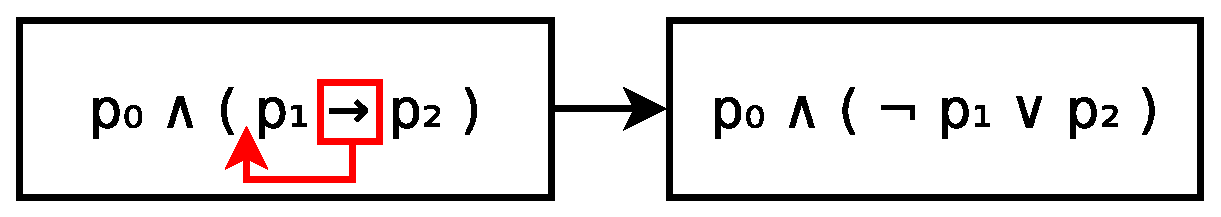
\includegraphics[width=.7\linewidth]{pics/implication.eps}
 \end{figure}

 In Pseudocode erfolgt dieser erste Schritt folgendermassen:
 \begin{lstlisting}
# 1. calculate p(A), the formula without implication
for each part of the formula:
    if formula[i] == implication:                     # found implication
        formula[i] = OR                               # replace it with OR
        if formula[i-1] == proposition or constant:
            formula.insert(i-1, NOT)
        elif formula[i-1] == ')':                     # brackets before implication
            index = beginning_of_brackets()           # search where brackets open
            formula.insert(index, NOT)
\end{lstlisting}
 
  \item Im zweiten Schritt wird $\nu(A)$ berechnet, welche Negationen nur direkt vor Propositonen oder Konstanten erlaubt ($\top, \bot$). Auch hier gibt es einige Ersetzungsregeln:
  \begin{itemize}
   \item $\neg \top \Rightarrow \bot$, $\neg \bot \Rightarrow \top$
   \item $\neg \neg A \Rightarrow A$
   \item $\neg (A \vee B) \Rightarrow \neg A \wedge \neg B$
   \item $\neg (A \wedge B) \Rightarrow \neg A \vee \neg B$
  \end{itemize}
\end{enumerate}

Nacheinander angewendet erhält man die Negationsnormalform, also:
\begin{equation}
nnf(A) = \nu(\rho(A))
\end{equation}

\subsection{Konjunktive Normalform (\textit{cnf})}
Ähnlich dazu wird die konjunktive Normalform erreicht, auch über zwei Schritte:

\begin{enumerate}
 \item $\sigma(A)$ wird berechnet, indem eine einfache Ersetzung vorgenommen wird:
 \begin{itemize}
  \item $\top \Rightarrow (p_0 \vee \neg p_0)$
  \item $\bot \Rightarrow (p_0 \wedge \neg p_0)$
 \end{itemize}

 \item Mit $\tau(A)$ werden dann alle $\vee$-Konjunktionen nur noch zwischen atomaren Propositionen erlaubt, und alle $\vee$, welche grössere Ausdrücke verbinden, werden ersetzt durch:
 \begin{itemize}
 \item $A \vee (B_1 \wedge B_2) \Rightarrow (A \vee B_1) \wedge (A \vee B_2)$
 \item $(A_1 \wedge A_2) \vee B \Rightarrow (A_1 \vee B) \wedge (A_2 \vee B)$
 \end{itemize}
 Hier kann keine simple Ersetzung erfolgen, da die Teile, welche ersetzt und dupliziert werden sollen, zuerst vom Rest der Formel isoliert werden müssen. Dazu wird die Suche verwendet, die im nächsten Abschnitt \ref{section:linear_search} vorgestellt wird. Erst wenn die Teile $A_1, A_2$ resp. $B_1, B_2$ identifiziert wurden, kann ein ``Umbau'' der Formel in die gewünschte Form stattfinden.
 Die Ersetzung bei einer etwas komplexeren Formel folgt auf diese Weise in mehreren Schritten, wovon der erste z.B. so aussieht:
 \begin{equation}
 (A_1 \wedge A_2) \vee (B1 \wedge B_2) \Rightarrow ((A_1 \wedge A_2) \vee B_1) \wedge ((A_1 \wedge A_2) \vee B_2)
 \end{equation}
 Zu beachten ist hier, dass das Verfahren keineswegs effizient oder optimiert ist, da bei den Ersetzungen im Worst Case die Länge der Formel bei jeder Ersetzung verdoppelt wird. So entsteht z.B. aus dem einfachen Ausdruck:
 \begin{equation}
 \top \vee \bot
 \end{equation}
 nach der Ersetzung der propositionalen Konstanten und der Ersetzungsregeln folgender äquivalente Ausdruck:
 \begin{equation}
 ( ( p_0 \vee \neg p_0 ) \vee p_0 ) \wedge ( ( p_0 \vee \neg p_0 ) \vee \neg p_0 )
 \end{equation}
\end{enumerate}

Zusammengefasst erhält man die konjunktive Normalform:
\begin{equation}
cnf(A) = \tau(\sigma(A))
\end{equation}

\subsection{Suche in Formel (\textit{linear\_search})}
\label{section:linear_search}
Ein wichtiger Bestandteil vieler Funktionen ist die lineare Suche. Ihr Zweck ist es, aufgrund einer öffnenden oder schliessenden Klammer \textit{den Teil der Formel zu finden, der die Klammer einschliesst}. Zum Beispiel muss bei einer Implikation klar sein, welcher Teil vor der Implikation genau beachtet werden muss, um die Implikation auszuwerten. Die lineare Suche nimmt als Parameter eine Position der Formel entgegen und eine Suchrichtung.
\begin{figure}[ht]
\centering
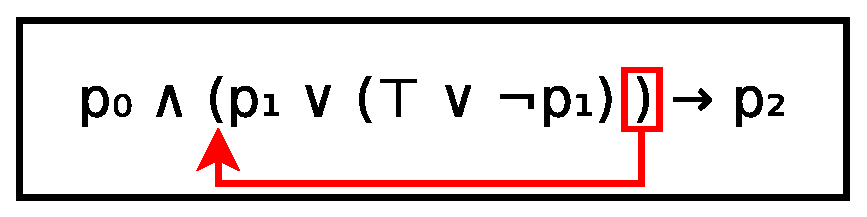
\includegraphics[width=.5\linewidth]{pics/linear_search.eps}
\end{figure}
Der Kern der linearen Suche besteht darin, sich lokal zu merken, auf welcher Ebene man sich befindet (welche Ebene das ist spielt global gesehen keine Rolle) und ausgehend von diesem Initialwert, der auf 0 gesetzt wird, wird je nach Klammer die lokale Ebene (\textit{local\_level}) herauf- oder heruntergesetzt, bis das entsprechende Gegenstück der Klammer gefunden wurde:
\begin{lstlisting}
while position not found:
    if pos == -1:             # beginning of formula
        return 0
    elif pos == len(formula): # end of formula
        return pos-1
    if formula[pos] == ')':   # one level up
        local_level -= 1
    elif formula[pos] == '(': # one level down
        local_level += 1
    if local_level == 0:      # again at level 0
            return pos        # return position
    pos += direction          # one step in search direction
\end{lstlisting}

\subsection{Einfache Evaluation (\textit{evaluate})}
Um die Überprüfung auf Erfüllbarkeit, also \textit{sat()}, vorzubereiten, wird zuerst ein Verfahren benötigt, um bei gegebenen Formeln, die nur aus porpositionalen Konstanten bestehen, festellen zu können ob diese zu \textit{true} oder \textit{false} evaluieren. Dabei werden Ausdrücke schrittweise ersetzt ($A$ steht für eine beliebige Formel):
 \begin{itemize}
  \item $\top \vee A \Rightarrow \top$, $A \vee \top \Rightarrow \top$
  \item $\bot \wedge A \Rightarrow \bot$, $A \wedge \bot \Rightarrow \bot$
  \item $\top \wedge \top \Rightarrow \top$
  \item $\bot \vee \bot \Rightarrow \bot$
 \end{itemize}
So kann eine Formel schrittweise vereinfacht werden:
\begin{align}
\bot \vee ( ( \top &\wedge \bot ) \wedge \top ) \\
\bot \vee &( \bot \wedge \top ) \\
\bot &\vee \bot \\
&\bot
\end{align}

\subsection{Erfüllbarkeit (\textit{sat})}
Der \textit{sat()}-Algorithmus wurde als einfache \textit{Brute Force}-Suche konzipiert, welche die erste gefundene Lösung zurückgibt, die sie findet. Er funktioniert wie folgt dargestellt, dabei wird als Beispiel die Formel 
\begin{equation}
p_0 \wedge ( \neg p_1 \vee ( p_3 \wedge p_0 ) )
\end{equation}
auf Erfüllbarkeit getestet.
\begin{enumerate}
 \item \textbf{Gesamtanzahl n der Propositionen feststellen} \\
 Zuerst wird festgestellt, wie viele unterschiedliche Propositionen in der Formel vorkommen. Im Beispiel sind dies 3: $p_0, p_1$ und $p_3$.
 \item \textbf{Iteration durch alle $2^n$ Möglichkeiten} \\
 Für den nächsten Schritt heisst dies, dass über alle $n=8$ Möglichkeiten iteriert wird. Dabei wird mit $n=0$ gestartet.
 \begin{enumerate}
 \item \textbf{Aktuelle Zahl in binäres Format umrechnen} \\
 Die Suche beginnt mit $n=0$, was binär $(000)_2$ entspricht. Bei steigendem $n$ ändert sich diese und läuft von $(001)_2$, $(010)_2$ etc. bis zu $(111)_2$.
 \item \textbf{Anstelle der Propositionen in Formel einsetzen} \\
 Nun wird der Reihe nach der entsprechende Wert eingesetzt. Dabei wird $0$ zu \textit{false} und $1$ zu \textit{true}. Im ersten Durchlauf wird also bei allen drei Propositionen \textit{false}, resp. $\bot$ eingesetzt:
 \begin{equation}
 \bot \wedge ( \neg \bot \vee ( \bot \wedge \bot ) )
 \end{equation}
 \item \textbf{Mit \textit{evaluate()} prüfen, ob die Formel zu \textit{true} evaluiert} \\
 Danach wird die nur noch aus porpositionalen Konstanten und Konjunktionen bestehende Formel der bereits erläuterten \textit{evaluate()}-Funktion übergeben. Evaluiert diese zu \textit{true}, wurde eine Lösung gefunden und die Belegung wird zurückgegeben. \\
 Im Beispiel evaluiert erst $(100)_2$, also $\top \wedge ( \neg \bot \vee ( \bot \wedge \top ) )$ zu \textit{true}.
 
 \end{enumerate}
\end{enumerate}

\subsection{Resolution (\textit{resolution})}
Aufbauend auf den Klauselmengen, die direkt aus der konjunktiven Normalform abgeleitet werden können, kann Resolution angewendet werden. Dieses Verfahren basiert auf einer Reihe von Schritten, die schliesslich dazu führen, dass entweder die leere Menge entsteht (in welchem Fall sie nicht erfüllbar ist) oder die Klauselmenge irreduzibel ist (in welchem Fall sie erfüllbar ist).

Die Resolution selbst ist relativ simpel und sieht im Code so aus:
\begin{lstlisting}
K = formula.clause_set()
length = 0
while len(K) != length:
    length = len(K)
    K = resolution_step(K)
    if [] in K: break
\end{lstlisting}
Erst im Resolutions-Schritt \textit{resolution\_step()}, der stets wiederholt wird, geschieht die eigentlich Resolution. Diese sieht vor, dass wenn ein Ausdruck eine beliebige Proposition $p$ wie auch ihre Negation $\neg p$ enthält, eine neue Klausel entsteht mit dem Rest der beiden betrachteten Klauseln.\\\\
Aus 
\begin{equation}
\{p_0, p_1\}, \{\neg p_0, \neg p_2\}
\end{equation}
entsteht somit die zusätzliche Klausel
\begin{equation}
\{p_1, \neg p_2\}
\end{equation}

\subsection{Deduktionsketten (\textit{dchains})}
Ausgehend von einer endlichen Anzahl Formeln sind Deduktionsketten eine Methode zur Prüfung auf Gültigkeit (Herleitbarkeit in PSC). Das Ziel ist es, das Verfahren zur Generierung der nächsten Sequenz von Kettengliedern so oft durchzuführen, bis entweder ein Axiom erreicht wird oder die Kette irreduzibel ist.\\
Dabei hat man folgende Möglichkeiten zur Manipulation der Deduktionsketten ($\Pi_n$ und $\Sigma_n$ sind beliebige Formeln):
\begin{align}
&\vee-\text{Zerlegung: } \Pi_n, A \vee B, \Sigma_n \Rightarrow \Pi_n, A, B, \Sigma_n \\
&\wedge-\text{Zerlegung: } \Pi_n, A \wedge B, \Sigma_n \Rightarrow \left\{ 
\begin{matrix} \Pi_n, A, \Sigma_n \\
\Pi_n, B, \Sigma_n
\end{matrix}
\right.
\end{align}
Dabei gibt es die folgenden zwei Axiome, bei denen die Kette aufhört und andere Zweige weiterverfolgt werden können:
\begin{align}
&\text{Identity-Axiom: } \Pi_n, \top, \Sigma_n \\
&\text{True-Axiom: } \Pi_n, p, \Delta_n, \neg p, \Sigma_n 
\end{align}
So wird aus einer Menge von Formeln ein Baum aufgebaut. Die initiale Menge entspricht dabei dem im Skript angesprochenen $\Gamma = \Gamma_0$, aus welchem die folgenden $\Gamma_1, \Gamma_2$ generiert werden.\\\\
Mit der \textit{Node}-Klasse wird so der Wurzelknoten instanziiert, und aus diesem alle folgenden Kinderknoten generiert. Entsprechend der Zerlegungen gibt es die folgenden Möglichkeiten für die nächste Generation:
\begin{itemize}
\item Die aktuelle Kette ist ein Axiom oder nicht weiter reduzierbar. In diesem Fall endet die Kette hier und der Ast hat keine weiteren Kinder.
\item Das am weitesten rechts zu verarbeitende Zeichen ist ein $\vee$. Die entsprechende Formel wird aufgeteilt und der Ast erhält einen weiteren Knoten als Nachkomme.
\item Das Zeichen ist ein $\wedge$. In diesem Fall teilt sich der Ast auf und es werden zwei neue Knoten generiert und als Kinder hinzugefügt.
\end{itemize}
\newpage \noindent Als Beispiel die Formel $p_0 \wedge ( \neg p_1 \vee p_2 )$: Diese wird in einem ersten Schritt aufgeteilt in $p_0$ und $\neg p_1 \vee p_2$.
\begin{figure}[ht]
\centering
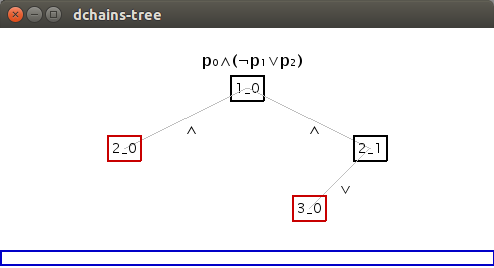
\includegraphics[width=.6\linewidth]{pics/tree1.png}
\end{figure}
Hier wird gleich sichtbar, dass der Knoten $p_0$, welcher in der Grafik links unten steht, irreduzibel ist, aber nicht in einem Axiom endet. \\
Ein anderes Beispiel mit einer gültigen Menge von Formeln ist das folgende. 
\begin{figure}[ht]
\centering
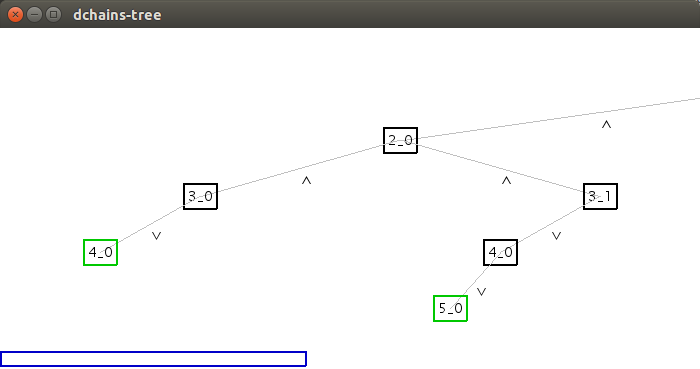
\includegraphics[width=.8\linewidth]{pics/tree2.png}
\end{figure}
Hier erfolgt eine durchgängige Prüfung aller Knoten, die meisten enden im True-Axion (grüne Markierung). \\\\
Die Koordinaten der einzelnen Knoten werden dabei durch einen einmaligen Durchlauf durch den Baum ermittelt. Hierbei wird je nach Tiefe des Baums die maximale Anzahl der Knoten auf dieser Ebene berechnet und anschliessend der Platz entsprechend verteilt, damit die Knoten auch beim Skalieren des Fensters das richtige Platzverhältnis aufweisen.

\section{Fehlerbehandlung}
\label{section:fehlerbehandlung}
\subsection{Exceptions}

\begin{itemize}
 \item \textbf{FormulaInvalidError} beschreibt eine ungültige Formel (wird im nächsten Abschnitt näher erläutert).
 \item \textbf{TimeOutError} entsteht wenn ein Berechnungsprozess (z.B. \textit{sat()}) eine festgelegte Zeitdauer (üblicherweise 5 Sekunden) überschreitet.
 \item \textbf{MaximalNestingSizeError} entsteht, wenn die maximale Tiefe einer Formel erreicht wurde. Die maximale Tiefe ist ein statischer Parameter, der beliebig eingestellt werden kann, um übermässige Verschachtelungen zu vermeiden.
 \item \textbf{UnexpectedTokenError} gibt an, dass ein Zeichen gefunden wurde, das an der Stelle nicht vorkommen dürfte. Dies kann z.B. die Implikation ($\rightarrow$) in einer Formel sein, die sich in Negationsnormalform befindet.
\end{itemize}

\subsection{Ungültige Formeln}
Besonderen Wert wurde darauf gelegt, ungültige Formeln zu erkennen und auch anzuzeigen, was an der jeweiligen Formel nicht gültig ist.
\begin{itemize}
\item \textbf{Ungültige Zeichen} \\
Beispiel: $p_0 a$
\item \textbf{Proposition ohne Index} \\
Beispiel: $p$
\item \textbf{Nicht verknüpfte Propositionen} \\
Beispiel: $p_0 p_1$
\item \textbf{Alleinstehende Indizes} \\
Beispiel: $p_0 \vee {}_2$
\item \textbf{Alleinstehende Negation} \\
Alleinstehende Negation vor einer Konjunktion oder am Schluss. \\
Beispiel: $p_0 \vee \neg$
\item \textbf{Ungültige Konjunktion} \\
Konjunktion an ungültiger Stelle, d.h. am Schluss, vor schliessender Klammer oder zwei Konjunktionen nacheinander. \\
Beispiel: $p_0 \wedge \vee p_1$
\item \textbf{Leere Formel} \\
Beispiel: $()$
\item \textbf{Gemischte $\wedge$ und $\vee$ auf selber Ebene} \\
Beispiel: $p_0 \wedge p_1 \vee p_2$
\item \textbf{Ungültige Implikation} \\
Beispiel: $\rightarrow p_0$
\item \textbf{Mehrere Implikationen auf selber Ebene} \\
Beispiel: $p_0 \rightarrow p_1 \rightarrow p_2$
\item \textbf{Ungleiche Anzahl öffnender und schliessender Klammern} \\
Beispiel: $((p_0 \wedge p_1) \vee p_2$
\item \textbf{Ungültige Klammernsetzung} \\
Beispiel: $(p_0 \vee p_1)) \wedge ((p_2)$
\end{itemize}

\section{Unit Tests}
Ziel der Unit Tests war einerseits, den Code auf Funktionalität zu testen, und andererseits, als Regressionstests bei neu hinzugefügten Funktionen sicherzustellen, dass die Funktionen noch so funktionieren wie sie sollten. Dazu wurden, aufbauend auf einfachen Beispielen, über komplexere Fälle bis hin zu Sonderfällen oder auftretenden Fehlern laufend Tests hinzugefügt, um eine stabile und robuste Umgebung sicherzustellen.\\\\
Als Beispiel die ersten drei von insgesamt 12 Tests für die Negationsnormalform:
\begin{lstlisting}
def test_nnf1(self):
    formula = Formula('p0')
    self.failUnless(formula.formula_nnf == u'p0')

def test_nnf2(self):
    formula = Formula('p0 IMPL p1')
    self.failUnless(formula.formula_nnf == u'NOT p0 OR p1')

def test_nnf3(self):
    formula = Formula('p0 AND p1 IMPL p2')
    self.failUnless(formula.formula_nnf == u'( NOT p0 OR NOT p1 ) OR p2')
...
\end{lstlisting}

Insgesamt wurden über 100 Tests (ca. 700 Zeilen Code) für die vorhandenen Funktionen geschrieben, mit dem Hauptaugenmerk auf den zentralen Funktionen wie den Normalformen, der Resolution und den Deduktionsketten.

\chapter{Fazit}  %====================================================================================
\section{Herausforderungen}
Eine grosse Herausforderung gleich zu Beginn war die interne Repräsentation einer Formel: Welche Eigenschaften sollte ein Formelobjekt haben? Sind eine Formel und ihre Negationsnormalform ein und dasselbe Objekt, oder zwei verschiedene Objekte? Schliesslich wurde die Variante gewählt, dass ein Objekt genau eine Formel repräsentiert, jedoch die verschiedenen Normalformen direkte Eigenschaften des Objekts sind und über Member-Variablen darauf zugegriffen werden kann (z.B. \textit{self.formula\_cnf}). So wird gewährleistet, dass auch die Eingabe des Benutzers selbst verfügbar bleibt (z.B. bei Meta-Variablen), andererseits aber für bestimmte Funktionen auch direkt die Normalformen abgerufen werden können, ohne weitere Objekte generieren zu müssen.\\
Eine weitere unerwartete Hürde lag in der syntaktischen Unklarheit, wie mit nicht-binären Formeln der Art:
\begin{equation}
p_0 \vee p_1 \vee p_2
\end{equation}
umzugehen ist. Hier wurde beschlossen, diese bei der \textit{pedantic}-Form in eine binäre Form zu zerlegen:
\begin{equation}
((p_0 \vee p_1) \vee p_2)
\end{equation}
Weiter war die Verarbeitung des Inputs nicht ganz trivial, da mit der Zuweisung von Meta-Variablen verschiedene Möglichkeiten bestehen, in einer Session zu arbeiten. Diese Struktur musste mehrfach überarbeitet werden, um wie auf aktuellem Stand auch verschachtelte Funktionen zulassen zu können. \\
Andere, kleinere Schwierigkeiten wie die Begrenzung der Rechenzeit beim \textit{sat()}-Algorithmus konnten über Methoden der Programmiersprache selbst gelöst werden (Zeitlimit der Berechnung).\\
Auch die Namensgebung und Darstellung der einzelnen Deduktionsketten konnte mit der grafischen Darstellung gelöst werden, ohne auf Details zu verzichten, da sich die Kette per Klick auf die einzelnen Knoten hervorholen lässt.

\section{Fazit}
Mit der Anwendung \textit{cp-logic} wurde ein Tool geschaffen, das einen Grossteil der besprochenen Methoden aus der Vorlesung \textit{Diskrete Mathematik und Logik} abdeckt und einem Publikum von Studenten und anderen Benutzern, welche die Verfahren gerne testen würden, zur Verfügung stellt. Dies geschieht auf einer nachvollziehbaren, skalierbaren Oberfläche, welche eine einfache Bedienung ermöglichen soll und ein einfaches, dem Skript sehr nahes Eingabesystem bietet.

Die Implementierung hat seine Einschränkungen, zum Beispiel die Laufzeit von \textit{sat()} oder die erwähnten ein, zwei fehlenden Funktionen, welche vernachlässigt wurden.
Der Fokus jedoch, die Deduktiosnketten und die Resolution, wurden erfolgreich umgesetzt und im Falle der Deduktionsketten noch grafisch interaktiv dargestellt. Abgedeckt durch eine breite Basis von Tests wurde der Code so einfach wie möglich gehalten und sollte deshalb für Erweiterungen und zukünftige Verbesserungen offen stehen.

\section{Ausblick}
Da der Aufbau bewusst modular gehalten wurde, wären Erweiterungen zu den bereits vorhandenen Funktionen einfach zu implementieren. Zum Beispiel könnte eine zusätzliche Klasse erstellt werden, welche Theorien, wie sie im Skript beschrieben werden, umsetzt und damit auch der \textit{sat()}-Algorithmus noch zusätzlich erweitert werden könnte, damit überprüfbar wäre, ob bestimmte Formeln \textit{with respect to theory T} erfüllbar wären.

Weiter wäre auch eine Web-Anwendung denkbar, bei der die Eingabe im Webbrowser erfolgt und die Verarbeitung zentral von einem Server übernommen würde. Um dies umsetzen zu können, müssten die momentan verwendeten Bibliotheken zur grafischen Darstellung und Interaktion ersetzt oder selbst geschrieben werden.

Eine andere Richtung wäre die Kombination des vorhandenen mit einem optimierten, leistungsstarken \textit{sat()}-Algorithmus, damit auch komplexere Formeln in sinnvoller Zeit abgearbeitet werden könnten.

\chapter*{Eidesstattliche Erklärung}
Ich versichere hiermit an Eides statt, dass ich die vorliegende Arbeit selbstständig verfasst, bisher weder ganz noch in Teilen als Prüfungsleistung vorgelegt und keine anderen als die angegebenen Hilfsmittel benutzt habe.
Sämtliche Stellen der Arbeit, die benutzten Werken oder Quellen aus dem Internet im Wortlaut oder dem Sinn nach entnommen sind, habe ich durch Quellenangaben kenntlich gemacht. Dies gilt auch für sämtliche Abbildungen. Ich bin mir bewusst, dass es sich bei Plagiarismus um schweres akademisches Fehlverhalten handelt, das Sanktionen nach sich zieht.\\\\
Bern, den \today

% Selbst unterschreiben!
%\begin{figure}[h]
%\includegraphics[width=0.3\textwidth]{pics/sign}
%\end{figure}
\end{document}